\PassOptionsToPackage{unicode=true}{hyperref} % options for packages loaded elsewhere
\PassOptionsToPackage{hyphens}{url}
%
\documentclass[]{article}
\usepackage{lmodern}
\usepackage{amssymb,amsmath}
\usepackage{ifxetex,ifluatex}
\usepackage{fixltx2e} % provides \textsubscript
\ifnum 0\ifxetex 1\fi\ifluatex 1\fi=0 % if pdftex
  \usepackage[T1]{fontenc}
  \usepackage[utf8]{inputenc}
  \usepackage{textcomp} % provides euro and other symbols
\else % if luatex or xelatex
  \usepackage{unicode-math}
  \defaultfontfeatures{Ligatures=TeX,Scale=MatchLowercase}
\fi
% use upquote if available, for straight quotes in verbatim environments
\IfFileExists{upquote.sty}{\usepackage{upquote}}{}
% use microtype if available
\IfFileExists{microtype.sty}{%
\usepackage[]{microtype}
\UseMicrotypeSet[protrusion]{basicmath} % disable protrusion for tt fonts
}{}
\IfFileExists{parskip.sty}{%
\usepackage{parskip}
}{% else
\setlength{\parindent}{0pt}
\setlength{\parskip}{6pt plus 2pt minus 1pt}
}
\usepackage{hyperref}
\hypersetup{
            pdftitle={Detecting interaction with unknown environmental covariate},
            pdfauthor={Ziang Zhang},
            pdfborder={0 0 0},
            breaklinks=true}
\urlstyle{same}  % don't use monospace font for urls
\usepackage[margin=1in]{geometry}
\usepackage{color}
\usepackage{fancyvrb}
\newcommand{\VerbBar}{|}
\newcommand{\VERB}{\Verb[commandchars=\\\{\}]}
\DefineVerbatimEnvironment{Highlighting}{Verbatim}{commandchars=\\\{\}}
% Add ',fontsize=\small' for more characters per line
\usepackage{framed}
\definecolor{shadecolor}{RGB}{248,248,248}
\newenvironment{Shaded}{\begin{snugshade}}{\end{snugshade}}
\newcommand{\AlertTok}[1]{\textcolor[rgb]{0.94,0.16,0.16}{#1}}
\newcommand{\AnnotationTok}[1]{\textcolor[rgb]{0.56,0.35,0.01}{\textbf{\textit{#1}}}}
\newcommand{\AttributeTok}[1]{\textcolor[rgb]{0.77,0.63,0.00}{#1}}
\newcommand{\BaseNTok}[1]{\textcolor[rgb]{0.00,0.00,0.81}{#1}}
\newcommand{\BuiltInTok}[1]{#1}
\newcommand{\CharTok}[1]{\textcolor[rgb]{0.31,0.60,0.02}{#1}}
\newcommand{\CommentTok}[1]{\textcolor[rgb]{0.56,0.35,0.01}{\textit{#1}}}
\newcommand{\CommentVarTok}[1]{\textcolor[rgb]{0.56,0.35,0.01}{\textbf{\textit{#1}}}}
\newcommand{\ConstantTok}[1]{\textcolor[rgb]{0.00,0.00,0.00}{#1}}
\newcommand{\ControlFlowTok}[1]{\textcolor[rgb]{0.13,0.29,0.53}{\textbf{#1}}}
\newcommand{\DataTypeTok}[1]{\textcolor[rgb]{0.13,0.29,0.53}{#1}}
\newcommand{\DecValTok}[1]{\textcolor[rgb]{0.00,0.00,0.81}{#1}}
\newcommand{\DocumentationTok}[1]{\textcolor[rgb]{0.56,0.35,0.01}{\textbf{\textit{#1}}}}
\newcommand{\ErrorTok}[1]{\textcolor[rgb]{0.64,0.00,0.00}{\textbf{#1}}}
\newcommand{\ExtensionTok}[1]{#1}
\newcommand{\FloatTok}[1]{\textcolor[rgb]{0.00,0.00,0.81}{#1}}
\newcommand{\FunctionTok}[1]{\textcolor[rgb]{0.00,0.00,0.00}{#1}}
\newcommand{\ImportTok}[1]{#1}
\newcommand{\InformationTok}[1]{\textcolor[rgb]{0.56,0.35,0.01}{\textbf{\textit{#1}}}}
\newcommand{\KeywordTok}[1]{\textcolor[rgb]{0.13,0.29,0.53}{\textbf{#1}}}
\newcommand{\NormalTok}[1]{#1}
\newcommand{\OperatorTok}[1]{\textcolor[rgb]{0.81,0.36,0.00}{\textbf{#1}}}
\newcommand{\OtherTok}[1]{\textcolor[rgb]{0.56,0.35,0.01}{#1}}
\newcommand{\PreprocessorTok}[1]{\textcolor[rgb]{0.56,0.35,0.01}{\textit{#1}}}
\newcommand{\RegionMarkerTok}[1]{#1}
\newcommand{\SpecialCharTok}[1]{\textcolor[rgb]{0.00,0.00,0.00}{#1}}
\newcommand{\SpecialStringTok}[1]{\textcolor[rgb]{0.31,0.60,0.02}{#1}}
\newcommand{\StringTok}[1]{\textcolor[rgb]{0.31,0.60,0.02}{#1}}
\newcommand{\VariableTok}[1]{\textcolor[rgb]{0.00,0.00,0.00}{#1}}
\newcommand{\VerbatimStringTok}[1]{\textcolor[rgb]{0.31,0.60,0.02}{#1}}
\newcommand{\WarningTok}[1]{\textcolor[rgb]{0.56,0.35,0.01}{\textbf{\textit{#1}}}}
\usepackage{graphicx,grffile}
\makeatletter
\def\maxwidth{\ifdim\Gin@nat@width>\linewidth\linewidth\else\Gin@nat@width\fi}
\def\maxheight{\ifdim\Gin@nat@height>\textheight\textheight\else\Gin@nat@height\fi}
\makeatother
% Scale images if necessary, so that they will not overflow the page
% margins by default, and it is still possible to overwrite the defaults
% using explicit options in \includegraphics[width, height, ...]{}
\setkeys{Gin}{width=\maxwidth,height=\maxheight,keepaspectratio}
\setlength{\emergencystretch}{3em}  % prevent overfull lines
\providecommand{\tightlist}{%
  \setlength{\itemsep}{0pt}\setlength{\parskip}{0pt}}
\setcounter{secnumdepth}{5}
% Redefines (sub)paragraphs to behave more like sections
\ifx\paragraph\undefined\else
\let\oldparagraph\paragraph
\renewcommand{\paragraph}[1]{\oldparagraph{#1}\mbox{}}
\fi
\ifx\subparagraph\undefined\else
\let\oldsubparagraph\subparagraph
\renewcommand{\subparagraph}[1]{\oldsubparagraph{#1}\mbox{}}
\fi

% set default figure placement to htbp
\makeatletter
\def\fps@figure{htbp}
\makeatother


\title{Detecting interaction with unknown environmental covariate}
\author{Ziang Zhang}
\date{15/10/2020}

\begin{document}
\maketitle

\hypertarget{summary-of-current-idea}{%
\section{Summary of current idea:}\label{summary-of-current-idea}}

\hypertarget{latent-model-for-binary-data}{%
\subsection{Latent Model for binary
data}\label{latent-model-for-binary-data}}

For binary response variable, it is often assumed that the reponse
variable \(y_i\) conditioning on the regressors \(G_1,G_2\) come from a
latent model such that: \begin{equation}\label{eqn:latentformulation}
\begin{aligned}
Y_i^* &= \beta_0 + \beta_1 G_1 + \beta_2 G_2 + \epsilon_i \\
Y_i &= I\{Y_i^*>0\} \\
\end{aligned}
\end{equation}

The unobserved latent variable \(Y_i^*\) determines whether the observed
response variable \(Y_i\) is 0 or 1. The error term \(\epsilon_i\) in
\(Y_i^*\) needs to have a completely known distribution, which can be
\(\text{N}(0,1)\) for the model to become a probit model, or a logistic
distribution with mean 0 and variance 3.28 for the model to become a
logistic regression model.

\hypertarget{potential-method-1-by-checking-linearity}{%
\subsection{Potential Method 1: By checking
linearity:}\label{potential-method-1-by-checking-linearity}}

\hypertarget{when-the-true-model-does-not-contain-interaction-with-environmental-factor}{%
\subsubsection{When the true model does not contain interaction with
environmental
factor}\label{when-the-true-model-does-not-contain-interaction-with-environmental-factor}}

First, consider that the true underlying model for the response variable
\(Y_i\) is a probit model without interaction effect, i.e:
\begin{equation}\label{eqn:probitModel}
\begin{aligned}
Y_i^* &= \beta_0 + \beta_1 G_1 + \beta_2 G_2 + \epsilon_i \\
Y_i &= I\{Y_i^*>0\} \\
\epsilon_i &\sim \text{N}(0,1)
\end{aligned}
\end{equation}

Therefore, it can be shown that:
\begin{equation}\label{eqn:probitModelLinearity}
\begin{aligned}
\text{P}(Y_i = 1| G_1, G_2) &= \text{P}(\epsilon_i > -(\beta_0 +\beta_1 G_1 + \beta_2 G_2)) \\
&= 1 - \Phi(-(\beta_0 + \beta_1 G_1 + \beta_2 G_2)) \\
&= \Phi(\beta_0 + \beta_1 G_1 + \beta_2 G_2)
\end{aligned}
\end{equation} Where \(\Phi(.)\) denote the CDF function of standard
normal distribution. Therefore,
\(\Phi^{-1}\bigg(\text{P}(Y_i = 1|G_1,G_2)\bigg)\) shoud be a linear
function of both \(G_1\) and \(G_2\).

\hypertarget{when-the-true-model-does-contain-gene-environment-interaction}{%
\subsubsection{When the true model does contain gene-environment
interaction}\label{when-the-true-model-does-contain-gene-environment-interaction}}

Assume for simplicity that \(E_i\) the environmental variable has a
normal distribution with mean \(\mu_E\) and variance \(\sigma_E^2\), and
suppose that the true underlying model is:
\begin{equation}\label{eqn:probitModelWithInteraction}
\begin{aligned}
Y_i^* &= \beta_0 + \beta_1 G_1 + \beta_2 G_2 + \beta_3 G_1 \times E + \epsilon_i \\
Y_i &= I\{Y_i^*>0\} \\
\epsilon_i &\sim \text{N}(0,1)
\end{aligned}
\end{equation}

Furthermore, we can compute that:
\begin{equation}\label{eqn:probitModelWithInteraction_MeanVar}
\begin{aligned}
\text{E}(Y_i^*|G_1,G_2) &= \beta_0 + (\beta_1 + \beta_3 \mu_E)G_1 + \beta_2 G_2 \\
\text{Var}(Y_i^*|G_1,G_2) &= (\beta_3 G_1)^2 \sigma_E^2 + 1 \\
Y_i^*|G_1, G_2 &\sim \text{N}\bigg(\beta_0 + (\beta_1 + \beta_3 \mu_E)G_1 + \beta_2 G_2,  \big(\beta_3 G_1\big)^2 \sigma_E^2 + 1\bigg)
\end{aligned}
\end{equation}

That implies that the probability we get a case for different levels of
\(G_1\) and \(G_2\) will be:
\begin{equation}\label{eqn:probitModelWithInteraction_Prob} 
\begin{aligned} 
\text{P}(Y = 1 | G_1, G_2) &= \text{P}(Y^* > 0| G_1, G_2) \\ 
                           &= \text{P}(\frac{Y^*  - \text{E}(Y^* |G_1,G_2)}{\sqrt{\text{Var}(Y^* |G_1,G_2)}} > \frac{-\text{E}(Y^* |G_1,G_2)}{\sqrt{\text{Var}(Y^* |G_1,G_2)}}) \\
                           &= \Phi \bigg( \frac{\text{E}(Y^* |G_1,G_2)}{\sqrt{\text{Var}(Y^* |G_1,G_2)}} \bigg)
\end{aligned}
\end{equation}

Therefore, applying the inverse CDF on both sides, we get
\[\Phi^{-1} \bigg(\text{P}(Y = 1 | G_1, G_2) \bigg) = \frac{\beta_0+(\beta_1 + \beta_3 \mu_E)G_1 + \beta_2 G_2}{\sqrt{(\beta_3^2 G_1^2 \sigma_E^2 + 1)}} \].

This is not a linear function of \(G_1\), but is a linear function of
\(G_2\).

\begin{enumerate}
\item If the true underlying model also contains another regressor $Z$ but $Z$ is uncorrelated with $G_2$ for example. Then eventhough ignoring that regressor breaks the structural assumption of probit model, so that the fitted model without $Z$ is no longer a probit model (since now $\epsilon$ does not follow standard normal), but $\Phi^{-1}(\text{P}(Y_i = 1|G_1,G_2))$ will still be a linear function of $G_2$. So detecting based on the linearity of $\Phi^{-1}\text{P}$ will not be affected by omitted exogenous regressors.
\item Since $P(Y_i = 1|G_1,G_2)$ is actually unknown in practice, we can estimate it using the sample proportion $\hat{P}(Y = 1|G_1 = g_1,G_2 = g_2) = \frac{\sum_{i=1}^{n} \text{I}\{y_i =1,G_{1i} = g_1, G_{2i} = g_2\}}{\sum_{i=1}^{n}  \text{I}\{G_{1i} = g_1, G_{2i} = g_2\}}$. We shouldn't use the fitted model to estimate them since our fitted model may be wrong.
\item The reason we used probit model instead of logistic model here is that assuming $E$ follows normal distribution, $Y^*|G_1,G_2$ will still be normal if we omit the interaction term, since linear combination of normal is normal. But assuming $E$ follows logistic distribution does not imply that $Y^*|G_1,G_2$ will be logistically distributed as logistic distribution is not closed under linear combination. However, based on the literatures, it seems like probit model and logistic model have really closed results in real applications.
\item If this method is feasible, I will try to find a test statistic that has a nice asymptotic null distribution for the testing of linearity.
\end{enumerate}

\hypertarget{potential-method-2-by-modeling-the-interaction-term-as-a-random-slope}{%
\subsection{Potential Method 2: By modeling the interaction term as a
random
slope:}\label{potential-method-2-by-modeling-the-interaction-term-as-a-random-slope}}

First, let's rewrite our previous latent variable specification:
\begin{equation}\label{eqn:latentformulationRandomSlope}
\begin{aligned}
Y_i^* &= \beta_0 + \beta_1 G_1 + \beta_2 G_2 + \beta_3 G_1 \times E_i + \epsilon_i \\
      &= \beta_0 + \beta_1 G_1 + \beta_2 G_2 + U_i * G_1 + \epsilon_i \\
Y_i &= I\{Y_i^*>0\} \\
U_i &= \beta_3 * E_i
\end{aligned}
\end{equation}

Here \(U_i\) can be thought as a random effect (random slope), being
drawn from distribution \(\text{N}(0,\sigma_u^2)\). Notice that
\(\sigma_u^2 = \beta_3^2\sigma_E^2\). Therefore, testing for
\(\beta_3 =0\) is equivalent to testing \(\sigma_u^2 = 0\) for the
random effects. In this case, we do not need to restrict our
distribution to the probit model anymore. Since both probit model and
logistic model are flexible enough to incorporate an observations-level
random slopes. (There shouldn't be any identifiability problem with have
too many random slopes(same number as observations), as including an
observations-level random intercepts is a common trick to account for
overdispersion in Poisson regression.)

\hypertarget{test-statistic-for-method-1}{%
\subsection{Test Statistic for Method
1:}\label{test-statistic-for-method-1}}

Let \(\hat{p_{ij}}\) denote the sample proportion of cases in the group
with \(G_1 = i\) and \(G_2 = j\), then we know that \(\hat{p_{ij}}\)
will be independent across different i and j. Also, by CLT:
\[\hat{p_{ij}} \sim N(p_{ij},\frac{p_{ij}(1-p_{ij})}{n_{ij}})\] where
\(n_{ij}\) denote the number of observations in the (i,j) cell.

By delta method: we can obtain the distribution of
\(\Phi^{-1}(\hat{p_{ij}})\) being:
\[\Phi^{-1}(\hat{p_{ij}}) \sim N\bigg(\Phi^{-1}(p_{ij}),\frac{1}{\phi(\Phi^{-1}(p_{ij}))^2}\frac{p_{ij}(1-p_{ij})}{n_{ij}}\bigg)\]
where \(\phi\) denotes the density of a standard normal.

Let \(Z_{ij} = \Phi^{-1}(\hat{p_{ij}})\). The variance of \(Z_{ij}\) can
be estimated as
\(v_{ij} = \frac{1}{\phi(\Phi^{-1}(\hat{p_{ij}}))^2}\frac{\hat{p_{ij}}(1-\hat{p_{ij}})}{n_{ij}}\),
which is simply plugging \(\hat{p_{ij}}\) for the unknown true
probability \(p_{ij}\). Let
\(S_1 = a_0(Z_{10}-Z_{00}) + a_1(Z_{11}-Z_{01}) + a_2(Z_{12}-Z_{02})\)
and
\(S_2 = a_0(Z_{20}-Z_{10}) + a_1(Z_{21}-Z_{11}) + a_2(Z_{22}-Z_{12})\),
where \(a_i\) is weight given to each difference term, such that
\(\sum_{i=0}^2 a_i =0\). If the allele frequency of \(G_1\) or \(G_2\)
is known. Then \(a_i = P(G_2 =i)\) when we are testing for the
interaction of \(G_1\) with \(E\). So \(S_1\) and \(S_2\) will have a
nice interpretation being estimated expected effect of \(G_1\).

Under the null hypothesis that \(\beta_3 =0\) which means no interaction
between \(G_1\) and \(E\), we know that \(\Phi^{-1}(p_{ij})\) should be
linear in i. That is:
\(Z_{(i+1)j} - Z_{ij} \sim N(b_i,v_{(i+1)j} + v_{ij})\) for all j =
0,1,2. So:
\[S_1 \sim N\bigg(\sum_{i=0}^{2}a_ib_i,\sum_{i=0}^{2}a_i^2(v_{1i}+v_{0i})\bigg) \]

\[S_2 \sim N\bigg(\sum_{i=0}^{2}a_ib_i,\sum_{i=0}^{2}a_i^2(v_{2i}+v_{1i})\bigg) \]

with the covariance between \(S_1\) and \(S_2\) be denoted as C, which
can be computed as:
\[ C = \text{Cov}(S_1,S_2) = -\sum_{i=0}^{2}v_{1i}a_i^2 \]

That means, if the null hypothesis is true,
\[ T = \frac{(S_1-S_2)^2}{\sigma_{S_1}^2+\sigma_{S_2}^2 -2C} \sim X^2_{df=1}\].
We will reject the null hypothesis when \(T\) has a large value.

\hypertarget{simulation-study}{%
\subsubsection{Simulation Study:}\label{simulation-study}}

Let n = 3000, and allele frequencies for \(G_1\) and \(G_2\) being
\(p=0.6\) and assuming that HWE holds in the population. First, consider
the case when the true model does not have interaction between \(G_1\)
and \(E\), let \(\beta_0,\beta_1,\beta_2\) be \(-1.2,0.8,0.3\)
respectively.

\begin{Shaded}
\begin{Highlighting}[]
\KeywordTok{set.seed}\NormalTok{(}\DecValTok{123}\NormalTok{)}

\NormalTok{n =}\StringTok{ }\DecValTok{3000}
\NormalTok{p1 <-}\StringTok{ }\FloatTok{0.6}
\NormalTok{q1 <-}\StringTok{ }\FloatTok{0.4}

\NormalTok{p2 <-}\StringTok{ }\FloatTok{0.6}
\NormalTok{q2 <-}\StringTok{ }\FloatTok{0.4}


\CommentTok{##### Generate random genotype for G1 and G2, and a normal environmental factor that is unknown:}
\NormalTok{G1 =}\StringTok{ }\KeywordTok{apply}\NormalTok{(}\DataTypeTok{X =} \KeywordTok{rmultinom}\NormalTok{(n,}\DecValTok{1}\NormalTok{,}\DataTypeTok{prob =} \KeywordTok{c}\NormalTok{(p1}\OperatorTok{^}\DecValTok{2}\NormalTok{,}\DecValTok{2}\OperatorTok{*}\NormalTok{p1}\OperatorTok{*}\NormalTok{q1,q1}\OperatorTok{^}\DecValTok{2}\NormalTok{)) }\OperatorTok{>}\StringTok{ }\DecValTok{0}\NormalTok{, }\DataTypeTok{FUN =} \StringTok{"which"}\NormalTok{,}\DataTypeTok{MARGIN =} \DecValTok{2}\NormalTok{) }\OperatorTok{-}\StringTok{ }\DecValTok{1}
\NormalTok{G2 =}\StringTok{ }\KeywordTok{apply}\NormalTok{(}\DataTypeTok{X =} \KeywordTok{rmultinom}\NormalTok{(n,}\DecValTok{1}\NormalTok{,}\DataTypeTok{prob =} \KeywordTok{c}\NormalTok{(p2}\OperatorTok{^}\DecValTok{2}\NormalTok{,}\DecValTok{2}\OperatorTok{*}\NormalTok{p2}\OperatorTok{*}\NormalTok{q2,q2}\OperatorTok{^}\DecValTok{2}\NormalTok{)) }\OperatorTok{>}\StringTok{ }\DecValTok{0}\NormalTok{, }\DataTypeTok{FUN =} \StringTok{"which"}\NormalTok{,}\DataTypeTok{MARGIN =} \DecValTok{2}\NormalTok{) }\OperatorTok{-}\StringTok{ }\DecValTok{1}


\CommentTok{### Case 1: If the true model is nicely additive without interaction (Assuming probit model, inverse normal CDF as link function)}
\NormalTok{beta0 <-}\StringTok{ }\FloatTok{-1.2}
\NormalTok{beta1 <-}\StringTok{ }\FloatTok{0.8}
\NormalTok{beta2 <-}\StringTok{ }\FloatTok{0.3}
\NormalTok{latent_y <-}\StringTok{ }\NormalTok{beta0 }\OperatorTok{+}\StringTok{ }\NormalTok{beta1}\OperatorTok{*}\NormalTok{G1 }\OperatorTok{+}\StringTok{ }\NormalTok{beta2}\OperatorTok{*}\NormalTok{G2 }\OperatorTok{+}\StringTok{ }\KeywordTok{rnorm}\NormalTok{(}\DataTypeTok{n =}\NormalTok{ n)}
\NormalTok{y <-}\StringTok{ }\KeywordTok{ifelse}\NormalTok{(latent_y }\OperatorTok{>}\StringTok{ }\DecValTok{0}\NormalTok{,}\DecValTok{1}\NormalTok{,}\DecValTok{0}\NormalTok{)}
\end{Highlighting}
\end{Shaded}

We can do a test for \(G_1\) first:

\begin{Shaded}
\begin{Highlighting}[]
\CommentTok{## Assuming that the true allele frequency of G2 is known}
\KeywordTok{test_lin}\NormalTok{(y,G1,G2, }\DataTypeTok{weight =} \KeywordTok{c}\NormalTok{(p2}\OperatorTok{^}\DecValTok{2}\NormalTok{,}\DecValTok{2}\OperatorTok{*}\NormalTok{p2}\OperatorTok{*}\NormalTok{q2,q2}\OperatorTok{^}\DecValTok{2}\NormalTok{))}
\end{Highlighting}
\end{Shaded}

\begin{verbatim}
## [1] 0.6514815
\end{verbatim}

\begin{Shaded}
\begin{Highlighting}[]
\CommentTok{## If the true allele frequency of G2 is unknown, use equal weights:}
\KeywordTok{test_lin}\NormalTok{(y,G1,G2)}
\end{Highlighting}
\end{Shaded}

\begin{verbatim}
## [1] 0.3209513
\end{verbatim}

The p-values from our hypothesis testing are larger than 0.05,
regardless whether we use the true allele frequency as the weights or
not. We can do the same procedure to test \(G_2\) as well, and the
results should not be significant as well:

\begin{Shaded}
\begin{Highlighting}[]
\CommentTok{## Assuming that the true allele frequency of G2 is known}
\KeywordTok{test_lin}\NormalTok{(y,G2,G1, }\DataTypeTok{weight =} \KeywordTok{c}\NormalTok{(p1}\OperatorTok{^}\DecValTok{2}\NormalTok{,}\DecValTok{2}\OperatorTok{*}\NormalTok{p1}\OperatorTok{*}\NormalTok{q1,q1}\OperatorTok{^}\DecValTok{2}\NormalTok{))}
\end{Highlighting}
\end{Shaded}

\begin{verbatim}
## [1] 0.3457912
\end{verbatim}

\begin{Shaded}
\begin{Highlighting}[]
\CommentTok{## If the true allele frequency of G2 is unknown, use equal weights:}
\KeywordTok{test_lin}\NormalTok{(y,G2,G1)}
\end{Highlighting}
\end{Shaded}

\begin{verbatim}
## [1] 0.258314
\end{verbatim}

The p-values also show that there should be no significant interaction
between \(G_2\) and \(E\).

We can check the behavior of the p-values from our test by doing this
simulation many times. Let's rerun the procedure for 1000 times and see
how the p-values behave: first using the true allele frequency as
weights:

\begin{Shaded}
\begin{Highlighting}[]
\NormalTok{p_values <-}\StringTok{ }\KeywordTok{simulate_test}\NormalTok{(}\DataTypeTok{n =} \DecValTok{3000}\NormalTok{, }\DataTypeTok{p1 =} \FloatTok{0.6}\NormalTok{, }\DataTypeTok{p2 =} \FloatTok{0.6}\NormalTok{, }\DataTypeTok{inter =} \OtherTok{FALSE}\NormalTok{, }\DataTypeTok{true_weight =}\NormalTok{ T,}\DataTypeTok{num_trial =} \DecValTok{1000}\NormalTok{,}\DataTypeTok{beta =} \KeywordTok{c}\NormalTok{(}\OperatorTok{-}\FloatTok{1.2}\NormalTok{,}\FloatTok{0.8}\NormalTok{,}\FloatTok{0.3}\NormalTok{,}\FloatTok{0.5}\NormalTok{))}
\KeywordTok{hist}\NormalTok{(p_values,}\DataTypeTok{freq =}\NormalTok{ F,}\DataTypeTok{breaks =} \DecValTok{30}\NormalTok{)}
\end{Highlighting}
\end{Shaded}

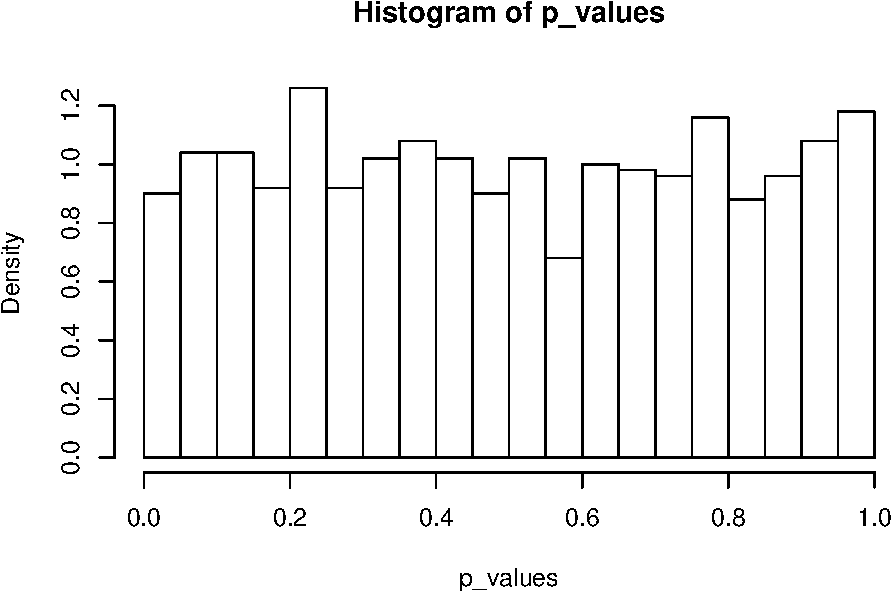
\includegraphics{stats-gene-progress-v2-_files/figure-latex/unnamed-chunk-5-1.pdf}

The histogram seems to be similar to \(\text{uniform}[0,1]\). Let's try
again using equal weights:

\begin{Shaded}
\begin{Highlighting}[]
\NormalTok{p_values <-}\StringTok{ }\KeywordTok{simulate_test}\NormalTok{(}\DataTypeTok{n =} \DecValTok{3000}\NormalTok{, }\DataTypeTok{p1 =} \FloatTok{0.6}\NormalTok{, }\DataTypeTok{p2 =} \FloatTok{0.6}\NormalTok{, }\DataTypeTok{inter =} \OtherTok{FALSE}\NormalTok{, }\DataTypeTok{true_weight =}\NormalTok{ F,}\DataTypeTok{num_trial =} \DecValTok{1000}\NormalTok{)}
\KeywordTok{hist}\NormalTok{(p_values,}\DataTypeTok{freq =}\NormalTok{ F,}\DataTypeTok{breaks =} \DecValTok{30}\NormalTok{)}
\end{Highlighting}
\end{Shaded}

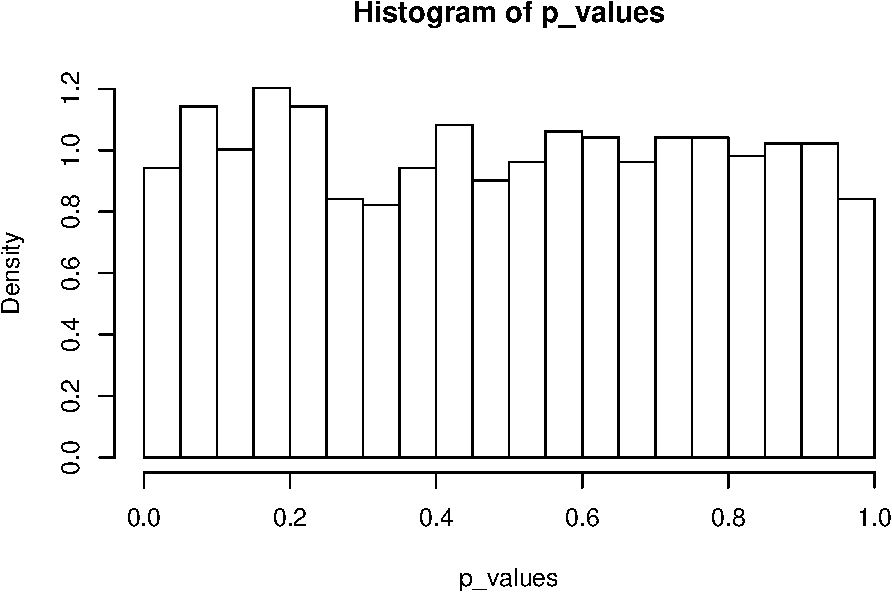
\includegraphics{stats-gene-progress-v2-_files/figure-latex/unnamed-chunk-6-1.pdf}

It still seems like \(\text{uniform}[0,1]\), so which weight to use
won't affect much when the null hypothesis is true.

Then, let's see whether our test can detect that when there is a
interaction \(G_1*E\) with \(\beta_3 = 0.5\) in our model, where
\(E \sim N(1,36)\).

\begin{Shaded}
\begin{Highlighting}[]
\KeywordTok{set.seed}\NormalTok{(}\DecValTok{123}\NormalTok{)}

\NormalTok{n =}\StringTok{ }\DecValTok{3000}
\NormalTok{p1 <-}\StringTok{ }\FloatTok{0.6}
\NormalTok{q1 <-}\StringTok{ }\FloatTok{0.4}

\NormalTok{p2 <-}\StringTok{ }\FloatTok{0.6}
\NormalTok{q2 <-}\StringTok{ }\FloatTok{0.4}


\CommentTok{##### Generate random genotype for G1 and G2, and a normal environmental factor that is unknown:}
\NormalTok{G1 =}\StringTok{ }\KeywordTok{apply}\NormalTok{(}\DataTypeTok{X =} \KeywordTok{rmultinom}\NormalTok{(n,}\DecValTok{1}\NormalTok{,}\DataTypeTok{prob =} \KeywordTok{c}\NormalTok{(p1}\OperatorTok{^}\DecValTok{2}\NormalTok{,}\DecValTok{2}\OperatorTok{*}\NormalTok{p1}\OperatorTok{*}\NormalTok{q1,q1}\OperatorTok{^}\DecValTok{2}\NormalTok{)) }\OperatorTok{>}\StringTok{ }\DecValTok{0}\NormalTok{, }\DataTypeTok{FUN =} \StringTok{"which"}\NormalTok{,}\DataTypeTok{MARGIN =} \DecValTok{2}\NormalTok{) }\OperatorTok{-}\StringTok{ }\DecValTok{1}
\NormalTok{G2 =}\StringTok{ }\KeywordTok{apply}\NormalTok{(}\DataTypeTok{X =} \KeywordTok{rmultinom}\NormalTok{(n,}\DecValTok{1}\NormalTok{,}\DataTypeTok{prob =} \KeywordTok{c}\NormalTok{(p2}\OperatorTok{^}\DecValTok{2}\NormalTok{,}\DecValTok{2}\OperatorTok{*}\NormalTok{p2}\OperatorTok{*}\NormalTok{q2,q2}\OperatorTok{^}\DecValTok{2}\NormalTok{)) }\OperatorTok{>}\StringTok{ }\DecValTok{0}\NormalTok{, }\DataTypeTok{FUN =} \StringTok{"which"}\NormalTok{,}\DataTypeTok{MARGIN =} \DecValTok{2}\NormalTok{) }\OperatorTok{-}\StringTok{ }\DecValTok{1}
\NormalTok{E <-}\StringTok{ }\KeywordTok{rnorm}\NormalTok{(n, }\DataTypeTok{mean =} \DecValTok{1}\NormalTok{, }\DataTypeTok{sd =} \DecValTok{6}\NormalTok{)}

\CommentTok{### Case 2: If the true model does have interaction}
\NormalTok{beta0 <-}\StringTok{ }\FloatTok{-1.2}
\NormalTok{beta1 <-}\StringTok{ }\FloatTok{0.8}
\NormalTok{beta2 <-}\StringTok{ }\FloatTok{0.3}
\NormalTok{beta3 <-}\StringTok{ }\FloatTok{0.5}
\NormalTok{latent_y <-}\StringTok{ }\NormalTok{beta0 }\OperatorTok{+}\StringTok{ }\NormalTok{beta1}\OperatorTok{*}\NormalTok{G1 }\OperatorTok{+}\StringTok{ }\NormalTok{beta2}\OperatorTok{*}\NormalTok{G2 }\OperatorTok{+}\StringTok{ }\NormalTok{beta3}\OperatorTok{*}\NormalTok{G1}\OperatorTok{*}\NormalTok{E }\OperatorTok{+}\StringTok{ }\KeywordTok{rnorm}\NormalTok{(}\DataTypeTok{n =}\NormalTok{ n)}
\NormalTok{y <-}\StringTok{ }\KeywordTok{ifelse}\NormalTok{(latent_y }\OperatorTok{>}\StringTok{ }\DecValTok{0}\NormalTok{,}\DecValTok{1}\NormalTok{,}\DecValTok{0}\NormalTok{)}

\CommentTok{### using true frequency as weight:}
\KeywordTok{test_lin}\NormalTok{(y,G1,G2, }\DataTypeTok{weight =} \KeywordTok{c}\NormalTok{(p2}\OperatorTok{^}\DecValTok{2}\NormalTok{,}\DecValTok{2}\OperatorTok{*}\NormalTok{p2}\OperatorTok{*}\NormalTok{q2,q2}\OperatorTok{^}\DecValTok{2}\NormalTok{))}
\end{Highlighting}
\end{Shaded}

\begin{verbatim}
## [1] 0
\end{verbatim}

\begin{Shaded}
\begin{Highlighting}[]
\CommentTok{### using equal weights:}
\KeywordTok{test_lin}\NormalTok{(y,G1,G2)}
\end{Highlighting}
\end{Shaded}

\begin{verbatim}
## [1] 2.174927e-13
\end{verbatim}

We can see that regardless whether we use the true frequency in our
hypothesis testing, we have strong evidence to say that \(G_1\) and
\(E\) have interaction. Let's test in this case, whether \(G_2\) has
interaction with \(E\):

\begin{Shaded}
\begin{Highlighting}[]
\KeywordTok{test_lin}\NormalTok{(y,G2,G1, }\DataTypeTok{weight =} \KeywordTok{c}\NormalTok{(p1}\OperatorTok{^}\DecValTok{2}\NormalTok{,}\DecValTok{2}\OperatorTok{*}\NormalTok{p1}\OperatorTok{*}\NormalTok{q1,q1}\OperatorTok{^}\DecValTok{2}\NormalTok{))}
\end{Highlighting}
\end{Shaded}

\begin{verbatim}
## [1] 0.1306443
\end{verbatim}

\begin{Shaded}
\begin{Highlighting}[]
\CommentTok{### using equal weights:}
\KeywordTok{test_lin}\NormalTok{(y,G2,G1)}
\end{Highlighting}
\end{Shaded}

\begin{verbatim}
## [1] 0.4002292
\end{verbatim}

Like we expected, in this case, we still have evidence to say that
\(G_2\) does not have interaction with \(E\).

Again, let's rerun this procedure 1000 times to see how powerful it is
in this setting:

\begin{Shaded}
\begin{Highlighting}[]
\NormalTok{p_values <-}\StringTok{ }\KeywordTok{simulate_test}\NormalTok{(}\DataTypeTok{n =} \DecValTok{3000}\NormalTok{, }\DataTypeTok{p1 =} \FloatTok{0.6}\NormalTok{, }\DataTypeTok{p2 =} \FloatTok{0.6}\NormalTok{, }\DataTypeTok{inter =} \OtherTok{TRUE}\NormalTok{, }\DataTypeTok{true_weight =}\NormalTok{ F,}\DataTypeTok{num_trial =} \DecValTok{1000}\NormalTok{,}\DataTypeTok{beta =} \KeywordTok{c}\NormalTok{(}\OperatorTok{-}\FloatTok{1.2}\NormalTok{,}\FloatTok{0.8}\NormalTok{,}\FloatTok{0.3}\NormalTok{,}\FloatTok{0.5}\NormalTok{))}
\KeywordTok{hist}\NormalTok{(p_values,}\DataTypeTok{freq =}\NormalTok{ F,}\DataTypeTok{breaks =} \DecValTok{30}\NormalTok{) }\CommentTok{### Using equal weights}
\end{Highlighting}
\end{Shaded}

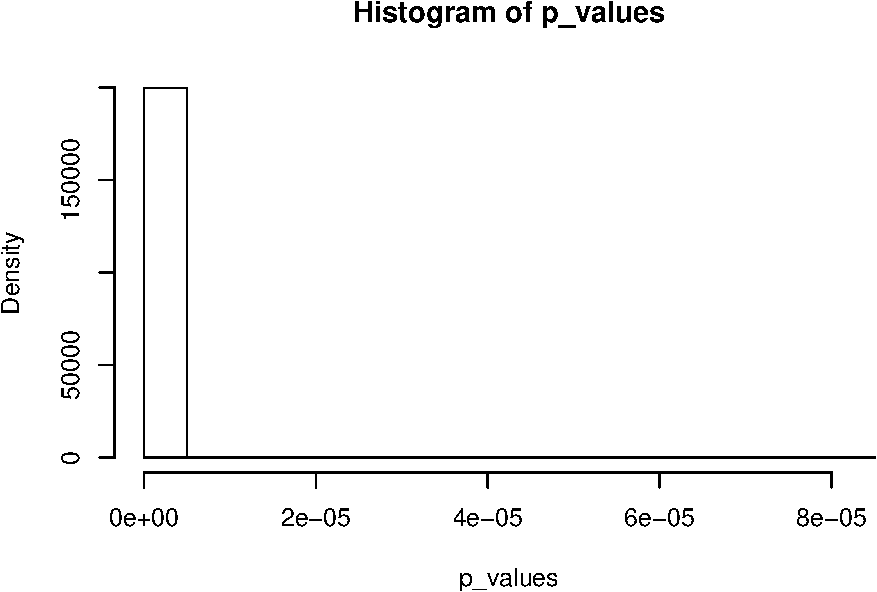
\includegraphics{stats-gene-progress-v2-_files/figure-latex/unnamed-chunk-9-1.pdf}

\begin{Shaded}
\begin{Highlighting}[]
\NormalTok{p_values <-}\StringTok{ }\KeywordTok{simulate_test}\NormalTok{(}\DataTypeTok{n =} \DecValTok{3000}\NormalTok{, }\DataTypeTok{p1 =} \FloatTok{0.6}\NormalTok{, }\DataTypeTok{p2 =} \FloatTok{0.6}\NormalTok{, }\DataTypeTok{inter =} \OtherTok{TRUE}\NormalTok{, }\DataTypeTok{true_weight =}\NormalTok{ T,}\DataTypeTok{num_trial =} \DecValTok{1000}\NormalTok{,}\DataTypeTok{beta =} \KeywordTok{c}\NormalTok{(}\OperatorTok{-}\FloatTok{1.2}\NormalTok{,}\FloatTok{0.8}\NormalTok{,}\FloatTok{0.3}\NormalTok{,}\FloatTok{0.5}\NormalTok{))}
\KeywordTok{hist}\NormalTok{(p_values,}\DataTypeTok{freq =}\NormalTok{ F,}\DataTypeTok{breaks =} \DecValTok{30}\NormalTok{) }\CommentTok{### Using true frequency}
\end{Highlighting}
\end{Shaded}

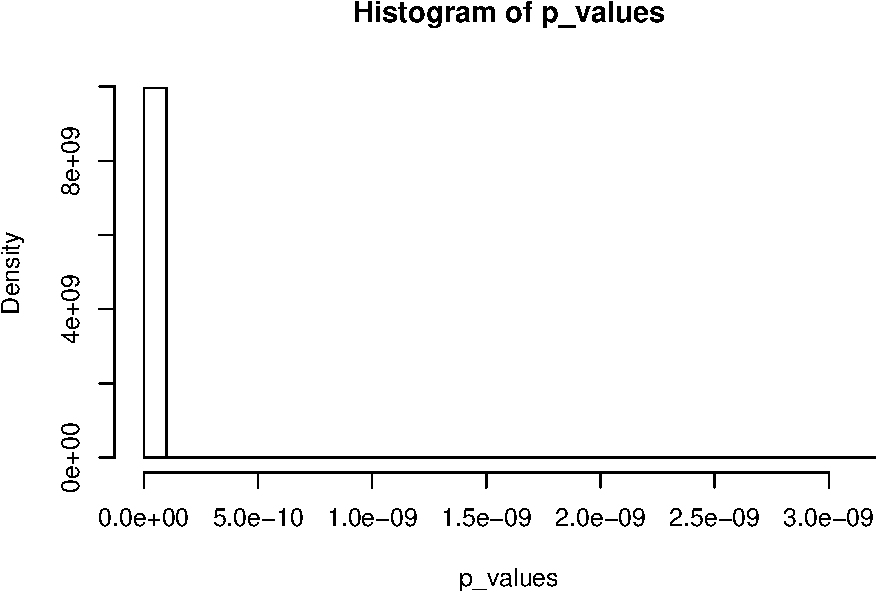
\includegraphics{stats-gene-progress-v2-_files/figure-latex/unnamed-chunk-9-2.pdf}

Regardless which weights being used, the distribution of p-values show
that under this setting, the procedure has enough power to detect the
interaction for all the 1000 simulations.

\hypertarget{difference-between-two-potential-methods}{%
\subsection{Difference between two potential
methods}\label{difference-between-two-potential-methods}}

\begin{enumerate}
\item The first method relies on the assumption that the true underlying model is probit model, and the distribution of $E$ is normal. These assumptions shouldn't be too restrictive as it is said in the literature that probit model and logistic model tend to give similar results. However, the second method can be used for both probit model and logistic model. The only assumption in the second method is that $E$ follows a normal distribution.
\item The next step for the first method is to develop a test statistic for testing the linearity. While for the second method, it seems like there are plenty of tools of testing at boudnary to test $\sigma_u = 0$, using likelihood ratio. It seems like in the second method, jointly testing for the main effect and interaction effect 
\item For the simulations of sample size 300000, the first method is very efficent to compute as it basically just computes nine sample proportions and compute their difference. If we can find a good test statistic for this, the hypothesis testing will be efficient to carry out and scale to larger sample. The second method takes a very long time to converge when the interaction is actually present in the model, and lme4 tends to give some warnings about the potential convergence problems if a probit model is fitted and underlying model has the interaction effect. For a larger sample with more regressors, the computational loads will be bigger for the second method.

\end{enumerate}

\end{document}
